%; whizzy paragraph -pdf xpdf -latex ./whizzypdfptex.sh
%; whizzy-paragraph "^\\\\begin{frame}\\|\\\\emtext"
% latex beamer presentation.
% platex, latex-beamer でコンパイルすることを想定。 

%     Tokyo Debian Meeting resources
%     Copyright (C) 2012 Junichi Uekawa

%     This program is free software; you can redistribute it and/or modify
%     it under the terms of the GNU General Public License as published by
%     the Free Software Foundation; either version 2 of the License, or
%     (at your option) any later version.

%     This program is distributed in the hope that it will be useful,
%     but WITHOUT ANY WARRANTY; without even the implied warreanty of
%     MERCHANTABILITY or FITNESS FOR A PARTICULAR PURPOSE.  See the
%     GNU General Public License for more details.

%     You should have received a copy of the GNU General Public License
%     along with this program; if not, write to the Free Software
%     Foundation, Inc., 51 Franklin St, Fifth Floor, Boston, MA  02110-1301 USA

\documentclass[cjk,dvipdfmx,12pt]{beamer}
\usetheme{Tokyo}
\usepackage{monthlypresentation}

%  preview (shell-command (concat "evince " (replace-regexp-in-string "tex$" "pdf"(buffer-file-name)) "&")) 
%  presentation (shell-command (concat "xpdf -fullscreen " (replace-regexp-in-string "tex$" "pdf"(buffer-file-name)) "&"))
%  presentation (shell-command (concat "evince " (replace-regexp-in-string "tex$" "pdf"(buffer-file-name)) "&"))

%http://www.naney.org/diki/dk/hyperref.html
%日本語EUC系環境の時
\AtBeginDvi{\special{pdf:tounicode EUC-UCS2}}
%シフトJIS系環境の時
%\AtBeginDvi{\special{pdf:tounicode 90ms-RKSJ-UCS2}}

\title{東京エリアDebian勉強会}
\subtitle{第96回 2013年1月度}
\author{上川純一\\dancer@debian.org}
\date{2013年1月19日}
\logo{
\includegraphics[width=8cm]{image200607/openlogo-light.eps}}

\begin{document}

\frame{\titlepage{}}

\begin{frame}{設営準備にご協力ください。}
会場設営よろしくおねがいします。
\end{frame}

\begin{frame}{Agenda}
\begin{minipage}[t]{0.45\hsize}
  \begin{itemize}
  \item 注意事項
	\begin{itemize}
	 \item 部屋内部以外の写真撮影
	\end{itemize}
   \item 最近あったDebian関連のイベント報告
	\begin{itemize}
        \item 第95回 東京エリアDebian勉強会
	\end{itemize}
   \item 事前課題紹介
 \end{itemize}
\end{minipage} 
\begin{minipage}[t]{0.45\hsize}
 \begin{itemize}
  \item Debian勉強会アンケート
  \item 2013-2015年を妄想する
  \item gdb python拡張その1
  \item 月刊Debhelper
 \end{itemize}
\end{minipage}
\end{frame}


\section{イベント報告}
\emtext{イベント報告}
\begin{frame}{第95回 東京エリアDebian勉強会}
\begin{itemize}
\item 開催場所は あんさんぶる荻窪でした。
\item im-configの紹介
\item 2012年のDebian勉強会の振り返り
\item DFSGと2012年改正著作権法についての発表
\end{itemize}
がありました。
\end{frame}

\section{DWN quiz}
\emtext{DWN quiz}
\begin{frame}{Debian 常識クイズ}

Debian の常識、もちろん知ってますよね?
知らないなんて恥ずかしくて、知らないとは言えないあんなことやこんなこと、
みんなで確認してみましょう。

今回の出題範囲は\url{debian-devel-announce@lists.debian.org},
\url{debian-devel@lists.debian.org} に投稿された
内容とDebian Project Newsなどからです。

\end{frame}

\subsection{問題}
%; whizzy-master ../debianmeetingresume201211.tex
% $B0J>e$N@_Dj$r$7$F$$$k$?$a!"$3$N%U%!%$%k$G(B M-x whizzytex $B$9$k$H!"(Bwhizzytex$B$,MxMQ$G$-$^$9!#(B
%

\santaku
{wiki.debian.org$B$G;H$o$l$F$$$?(Bwiki$B%7%9%F%`$N%=%U%H%&%'%"$NL>A0$O!)(B}
{pukiwiki}
{mine}
{moin}
{C}
{$B@?$K0d48$J$,$i!"(Bwiki.debian.org$B$,$3$NA0%/%i%C%/$5$l$?$h$&$G$9!#(B
$BB>$GF1$8EPO?%a!<%k%"%I%l%9$H%Q%9%o!<%I$NAH$r;H$C$F$$$k?M$O!"(B
$B$9$0$K%Q%9%o!<%I$rJQ$($?J}$,$h$$$G$7$g$&!#(B}

\santaku
{$B5nG/$NG/Kv$N(Bpopcon$BD4::$G(BNo.1$B$K51$$$?%W%i%C%H%U%)!<%`$O!)(B}
{$BEvA3(Barmel$B$@$m!)(B}
{i386}
{amd64}
{C}
{\url{http://popcon.debian.org/}$B$N%H%C%W%Z!<%8$K7k2L$N%0%i%U$,$"$j$^$9!#(B
 $B:#$^$G(BNo.1$B$r7h$a$F$$$?(Bi386$B$rG/Kv$G(Bamd64$B$,H4$-5n$C$?$h$&$G$9!#(B}

\santaku
{1$B7nF,$N(BDPN$B$GJs9p$N$"$C$?!"(Bwheezy$B$K;D$C$F$$$k(BRC$B%P%0$N?t$O(B1$B7n(B5$BF|;~E@$G$"$H2?8D!)(B}
{$B$"$H(B321$B8D(B}
{$B$"$H(B171$B8D(B}
{$B$"$H(B17$B8D(B}
{B}
{$B4JC1$KD>$;$k(B/$BB><#$l$P>!<j$K<#$j$=$&$b$N$r4^$s$G(B171$B8D!#<j$,$+$+$j$=$&$J$N$O(B
$B$@$$$?$$(B116$B8D$@$=$&$G$9!#(B}

\santaku
{$B:#G/(Bamazon$B$+$i(BDebian Project$B$X$$$/$i$+$N(BAWS$B$NMxMQ7t$r%9%]%s%5!<$7$F$b$i$C$?$=$&$J$N$G$9$,!"6b3[$K$9$k$H$*$$$/$i!)(B}
{8000USD}
{800USD}
{80000USD}
{A}
{$BF|K\1_$K$9$k$HLs(B72$BK|1_J,$NMxMQ7t!#(BQA$B$K$O==J,$H$N$3$H$G$7$?!#(B}












\section{事前課題}
\emtext{事前課題}
{\footnotesize
 %; whizzy-master ../debianmeetingresume201301.tex
% $B0J>e$N@_Dj$r$7$F$$$k$?$a!"$3$N%U%!%$%k$G(B M-x whizzytex $B$9$k$H!"(B
% whizzytex$B$,MxMQ$G$-$^$9(B

\begin{prework}{$B>e@n=c0l(B}

\preworksection{2013$BG/$NJY6/2q$GH/I=$7$?$$FbMF$r65$($F$/$@$5$$(B}
\preworksection{2015$BG/$G$O(BDebian$B$,$I$&$J$C$F$$$k$+$rBgC@$KM=A[$7$F$/$@$5$$(B}


\end{prework}

}

\section{Debian勉強会予約システムアンケート集計}
\emtext{Debian勉強会予約システムアンケート集計}

\begin{frame}{アンケートスコア}

\begin{figure}[h]
\begin{center}
  \includegraphics[angle=270,width=0.8\hsize]{image201301/enquete_boxplot.eps}

\end{center}
 \caption{毎回のスコアの分布}\label{fig:enquete-score-distribution}
\end{figure}
 
\end{frame}


\begin{frame}
 
\begin{figure}[h]
\begin{center}
 \includegraphics[angle=270,width=0.8\hsize]{image201301/raw_average_score_density.eps}

 \caption{すべての回を通しての平均点の分布}
 \label{fig:all-enquete-score-distribution}
\end{center}
\end{figure}

\end{frame}


\begin{frame}
\begin{figure}[h]
\begin{center}
 \includegraphics[angle=270,width=0.8\hsize]{image201301/score_hist_8.eps}

 \caption{あるユーザのつけたスコア分布}
 \label{fig:example-user-score-1}
\end{center}
\end{figure}
\end{frame}

\begin{frame}{ロースコアの例}
\begin{itemize}
 \item                 第71回東京エリアDebian勉強会.2010年12月勉強会.Debian.Miniconf.企画.2eca 
                                                                               2.333333 
 \item               第84回東京エリアDebian勉強会.2012年1月勉強会.事前課題紹介.2012年企画.f447 
                                                                               2.500000 
 \item 
       第84回東京エリアDebian勉強会.2012年1月勉強会.第3回月刊Debhelper.dh\_auto\_..dh\_build.f447 
                                                                               2.500000 

\end{itemize}
\end{frame}

\begin{frame}{ハイスコアの例}
\begin{itemize}
  \item 
      第71回東京エリアDebian勉強会.2010年12月勉強会.CACertの準備に何が必要か.2eca 
                                                                         4.600000 
 \item 
       第71回東京エリアDebian勉強会.2010年12月勉強会.俺のlibsaneが火をふくぜ.2eca 
                                                                         4.666667 
 \item 
                         第72回東京エリアDebian勉強会.2011年1月勉強会.Kinect.f456 
                                                                         4.875000 
 \item 
   第79回東京エリアDebian勉強会.2011年8月勉強会.Debianパッケージのビルド方法.5dff 
                                                                         5.000000 
 \item 
            第91回東京エリアDebian勉強会.2012年8月勉強会.DebianでC..11を使う.9796 
                                                                         4.666667 
 \item 
第91回東京エリアDebian勉強会.2012年8月勉強会.月刊.Debhelper.共有ライブラリ編.9796 
                                                                         5.000000 
 \item 
                  第95回東京エリアDebian勉強会.2012年12月勉強会.著作権法改正.3f15 
                                                                         4.750000 

\end{itemize}
\end{frame}

\section{2015年を妄想する}
\emtext{2015年を妄想する}
\begin{frame}{2015年を妄想する}
 
 { \tiny
\begin{tabular}[t]{|p{8.5em}|p{12em}|p{8em}|p{6em}|p{8em}|}
 \hline
 2011 &2012 & 2013 & 2014 & 2015 \\
 \hline

 %2011

 デスクトップパソコン終了の潮流。

 cpuコア単体では高速化しないように。

 webos終了のお知らせ。

 adobe flash復活のお知らせ(キタ), silverlight終了のお知らせ(台湾を除く)(続いてる?)

 squeezeリリース(おめでとう)

 ipv4割り当ての終了のお知らせ(キタ)

 地上波デジタル移行延長。

 btrfsまだ頑張る(fedora乙)

 java終了(sun java終了)

 open officeがoracle officeに(ナイ)

 &
 %2012

 ノートパソコンよりタブレットのほうが売れている。
 ノートパソコンではmacbookairが常識に。

 ノートパソコンでintelじゃないもの(mips/arm)が主流にはまだならず。タブレッ
 トのほうが主流。

 デスクトップ:ゲーム以外の用途では終了している。

 サーバ:個人レベルではVPS常識。企業ユースでもcloud か、vpsかを自前と比較
     検討する時代。データセンターを置く国を選べる時代。

 携帯電話:
 ガラパゴスの終焉。日本での携帯電話販売でもスマートフォンが50%を超えるように。
     ガラケー向けのネットバンクの提供が終了など、ガラケーからサービスが
     撤退し始める。
 LTE登場、普及しはじめたが、主流になっていない。
 softbankの二年契約はまだ続いている。sim freeへの道は耕されたがあたり前にならなかった。

 btrfsはまだ生き残っているがまだ使われてない?

     openstack で ceph 使う人もいる?

 mysqlからmariadbが派生。

 & 
 % 2013

コンシューマーはノートパソコンを買わなくなった。
ノートパソコンのかわりにスマートフォンを使っている。

スマートフォンが7インチくらいまで拡大、タブレットとは何だったのか。

自宅用のデスクトップパソコンのかわりに10インチくらいのタブレットを使うよ
	 うに。

サーバ:クラウドで処理するのが主流。python / ruby でコード書いていると
	 CPUが何かわからない。裏で動いているCPUは一般人は知らない。

ARMホストの仮想化技術が発達。

Oracle がメンテナンスする気がないのが明確になり、java リスクが顕著になる。

固定ゲーム機の終焉。

ゲームはARM。

 & 
 % 2014

Intel がまたARMに参入、もしくは省電力CPUを主力に切り替える。

気づいたら自作パソコン業界が終焉している。
セキュアブートが普及している。

AMD が ARM コアのCPUを出す。

Java が Oracle管理からはずれる。

スマートフォンの電池がガラケーなみに持つようになる。

電池消費が重要なアプリ選択の要素となる。
スポイトで充電できる、燃料電池が流行る。

ARメガネのプロトタイプが出てくる。

 & 
 % 2015

自作スマホの時代。
OpenHardwareがモバイルに移行する。
技適のパーツ認定基準というのができるようにがんばる。

自宅で回路が印刷できる機器が普及してCPUとかが印刷できるようになるといい
		 な。

タブレットが丸められるようになって巻物になっている。

AMD が x86 撤退。

ハードディスクを見たことがない人がいる。

データセンターを自前でもっているのは発電所を持っているところだけになる。

クラウドの法制度、免責事項、個人情報保護関連の問題が提起され、解決にむけ
		 てすすむ。
一種データセンタークラウド業者の要求規格が制定される。
ユーザ数何人以上は二種免許が必要とか。

データセンターヘイブンとよばれる国が存在する。


 \\

 \hline
 \end{tabular}

 }
\end{frame}

\begin{frame}{2013年の計画提案}

 手元の資料に書き出してみてください 
\end{frame}

\begin{frame}%{2013年の計画}

{
\begin{enumerate}
 \item 2013年の計画立案
 \item OSC 東京 nojima 
 \item UEFI・セキュアブートをDebianでどうやるか
 \item セキュアOS再入門
 \item Debianで自動化の夢は見れるか -- データセンターで OS のインストールからアプリのデプ
       ロイ、サービス公開まで
 \item amazon AWS での Debian 入門
 \item スイスでキャンプ
 \item Debian でスクリプト言語のパッケージ: perl, ruby, python
 \item Debian で apache 2.4: サーバ構築、Apache module プログラミング
 \item Raspberry Pi 、 SheevaBox、Freedombox は今
 \item 自由なFPGA
 \item 一年間の反省
\end{enumerate}
}
\end{frame}

\section{月刊Debhelper}
\emtext{月刊Debhelper}

\begin{frame}{今月のコマンド}
\Large
\begin{itemize}
\item dh\_gencontrol
\item dh\_listpackages
\end{itemize}

\end{frame}

\begin{frame}{dh\_gencontrol動作概要(その1)}

debian/controlファイル、debian/subversファイル、
debian/changelogファイルを用いて、
構築するバイナリパッケージに梱包するDEBIAN/controlファイル
と、debian/filesファイルを作る。

\end{frame}

\begin{frame}[containsverbatim]{バイナリパッケージの依存関係}

ソースパッケージのdebian/controlファイルに記載している、
バイナリパッケージの依存関係を示すフィールドに含まれる
\begin{itemize}
\item \verb!${misc:Depends}!
\item \verb!${shlibs:Depends}!等
\end{itemize}
の変数も、dh\_gencontrolによりdebian/subversを使って置き替える。

\end{frame}


\begin{frame}[containsverbatim]{DEBIAN/controlファイル(その1)}

xgalagaの例:
\begin{commandline}
Package: xgalaga
Version: 2.1.1.0-4
Architecture: amd64
Maintainer: Debian Games Team <pkg-games-devel@lists.alioth.debian.org>
Installed-Size: 690
Depends: libc6 (>= 2.7), libx11-6, libxext6, libxmu6, libxpm4, libxt6, libxxf86vm1
Section: games
Priority: optional
Homepage: http://sourceforge.net/projects/xgalaga/
Description: X version of the famous Galaga game
 A clone of the classic game Galaga for the X Window System.
 Xgalaga is a space-invader like game with additional features to produce
 a more interesting game.
\end{commandline}

\end{frame}

\begin{frame}[containsverbatim]{DEBIAN/controlファイル(その2)}

バイナリパッケージに関する基本情報が記載されている。

\begin{itemize}
\item バージョンとか、
\item どのアーキテクチャ用のファイルか、
\item 他のどのパッケージを必要としているか、
\item インストール後のサイズとか、
\item どのパッケージと競合するかとか
\end{itemize}
etc...
詳しくは、Debian Policy Manualや、man deb-controlを参照ください。
\end{frame}

\begin{frame}[containsverbatim]{DEBIAN/controlファイル(その3)}

バイナリパッケージがインストールされると、
\begin{itemize}
\item /var/lib/dpkg/status等
\end{itemize}

に溜め置かれ、dpkgコマンドの各操作の時に参照される。

\end{frame}

\begin{frame}{dh\_gencontrolの動作を図示すると}

\begin{figure}[h]
\begin{center}
 \includegraphics[width=0.8\hsize]{image201301/debhelper/dh-gencontrol-gen.eps}
\end{center}
\end{figure}

\end{frame}

\begin{frame}{dh\_listpackages}

 dh\_listpackagesコマンドは、debian/controlファイルを参照して、構築予定となる
バイナリパッケージの名前の一覧を得ます。

 なお、dh\_listpackagesは、dhコマンドから呼び出された場合には、
dhコマンドから引きついた情報を元に、構築予定のバイナリパッケージ
の一覧を得る事ができます。つまり、dhコマンドから呼び出される
他のdebhelperコマンドが、どんなパッケージに対して作用する予定
かを、dh\_listpackagesを使って知ることができます。

(例:Archtecture: i386指定とかのパッケージは、
amd64環境では構築候補としてリストされない等)

\end{frame}

\begin{frame}[containsverbatim]{dh\_listpackagesを動かすしてみた}

\begin{commandline}
$ apt-get source dpkg
$ cd dpkg-1.16.9
$ dh_listpackages
libdpkg-dev
dpkg
dpkg-dev
libdpkg-perl
dselect
$
\end{commandline}


\end{frame}

\begin{frame}[containsverbatim]{参考:debian/controlからパッケージ一覧抜いてみた}

\begin{commandline}
$ egrep '^Package' debian/control
Package: libdpkg-dev
Package: dpkg
Package: dpkg-dev
Package: libdpkg-perl
Package: dselect
$ 
\end{commandline}

とりあえず、実行した環境(amd64)と、debian/controlに
定義されているパッケージは、dpkgでは一致したようです。

\end{frame}

\begin{frame}{次回発表者は?}

\Large

\center{〜さんですー}

\end{frame}

\section{今後のイベント}
\emtext{今後のイベント}
\begin{frame}{今後のイベント}
\begin{itemize}
 \item 2013年2月 OSC Tokyo
 \item 2013年3月 Debian勉強会
\end{itemize}
\end{frame}

\section{今日の宴会場所}
\emtext{今日の宴会場所}
\begin{frame}{今日の宴会場所}
未定
\end{frame}

\end{document}

;;; Local Variables: ***
;;; outline-regexp: "\\([ 	]*\\\\\\(documentstyle\\|documentclass\\|emtext\\|section\\|begin{frame}\\)\\*?[ 	]*[[{]\\|[]+\\)" ***
;;; End: ***
